\section{Why predicted safety does not ensure competitive survival}
\label{sec:jesper-failures}
\contributionauthor{Jesper Eggers}
We audit selected actions at indices 1, 11, 21, and so forth using the
same engine reference, augmented with observed active explosions and
opponents blocking the first move. Future opponent actions and new bombs
remain unspecified. Against rule-based opponents, native selection has
zero unsafe choices among 5,401 recoverable observations, whereas the
learned RUEHL-mask variant has eleven among 978. All eleven precede
observed death within six steps. This is a descriptive association;
the sampling scheme and omitted opponent dynamics prevent interpreting
the reference as a complete attribution of deaths.

To investigate the native policy's losses, we replay its first episode,
seed 270920260, and audit every action. All 216 requested actions and
official outcomes match the primary run. Of the 216 observed states,
215 are recoverable; the reference finds a surviving continuation after
each selected first action in those states. The final state is already
unrecoverable. Figure~\ref{fig:jesper-native-failure}
shows why. At step 212, the agent places a bomb at $(8,15)$. At step 215,
it occupies $(10,15)$ and requests \texttt{RIGHT}, with a conditional
escape through $(11,15)$. An opponent at $(11,14)$ moves down into that
destination before the focal action executes. The movement becomes invalid.
At step 216, the focal agent remains at $(10,15)$, its bomb has timer zero,
and the opponent occupies the intended escape tile. The fallback selects
\texttt{LEFT} inside the imminent own-bomb blast, followed by self-destruction.
At step 215, \texttt{LEFT} also had a conditional escape. Binary viability
misses the routes' different exposure to interference; neither route
establishes a counterfactual winning policy.

Attack productivity is also limited. Native rule-based games contain
3,706 dropped bombs and 26 credited kills. Of 1,314 placements threatening
an opponent's current tile, only twelve satisfy the implementation's
predicted-trap test. Threatening a location rarely establishes a predicted
trap here. These are placement diagnostics, not verified trap outcomes,
and kills per bomb is not a success probability. Improving opponent-aware
escape and attack reasoning is therefore a more specific hypothesis than
simply increasing network size.

\begin{figure}[!htbp]
\centering
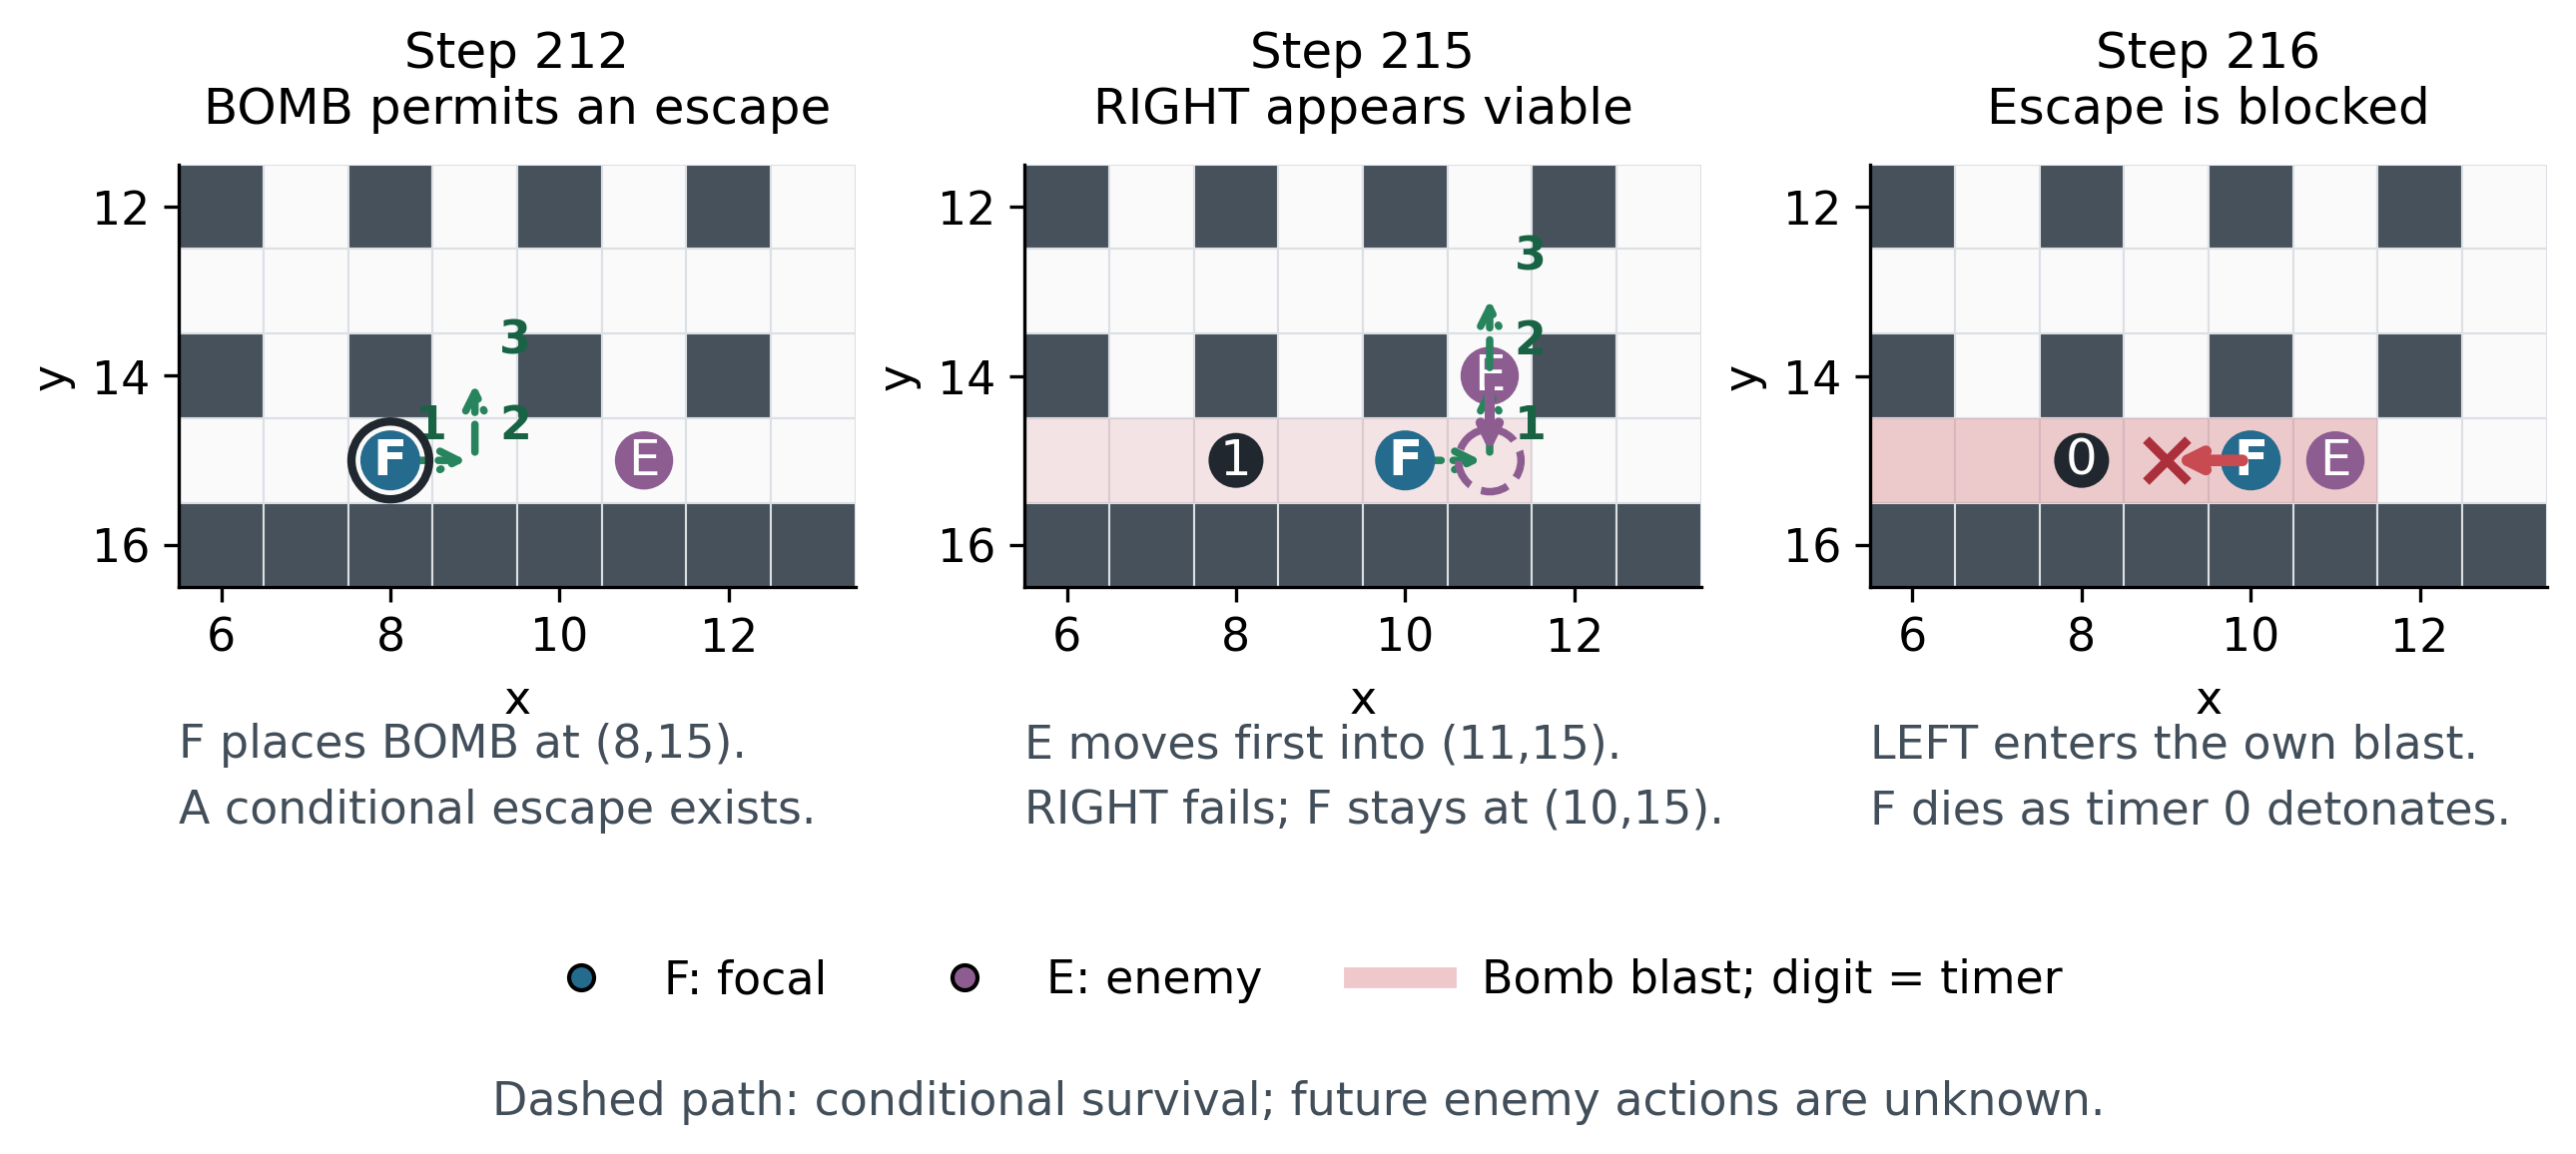
\includegraphics[width=\textwidth]{figures/native_gameplay_failure.png}
\caption{Recorded states from the first native-policy episode. Opponent
movement blocks a requested escape before it executes. Conditional
reachability and physical execution consequently diverge.}
\label{fig:jesper-native-failure}
\end{figure}
\FloatBarrier
